\documentclass[sigconf, nonacm]{acmart}

%% complete the rights form.
\setcopyright{none}

%% These commands are for a PROCEEDINGS abstract or paper.
\acmConference[Dundee Computing Honours Project '22]{Computing Honours Projects '22: The University of Dundee Computing Project Showcase: '22.}{2022}{Dundee, UK}


%%
%% end of the preamble, start of the body of the document source.
\begin{document}

%%
%% The "title" command has an optional parameter,
%% allowing the author to define a "short title" to be used in page headers.
\title{Code Quality}


\author{Christy McCarron}
\email{cswmccarron@dundee.ac.uk}
\affiliation{%
  \institution{University of Dundee}
  \city{Dundee}
  \state{Scotland}
  \country{UK}
}

%%
%% The abstract is a short summary of the work to be presented in the
%% article.

\begin{abstract}
Your abstract will go here.
\end{abstract}


%% A "teaser" image appears between the author and affiliation
%% information and the body of the document, and typically spans the
%% page.
\begin{teaserfigure}
  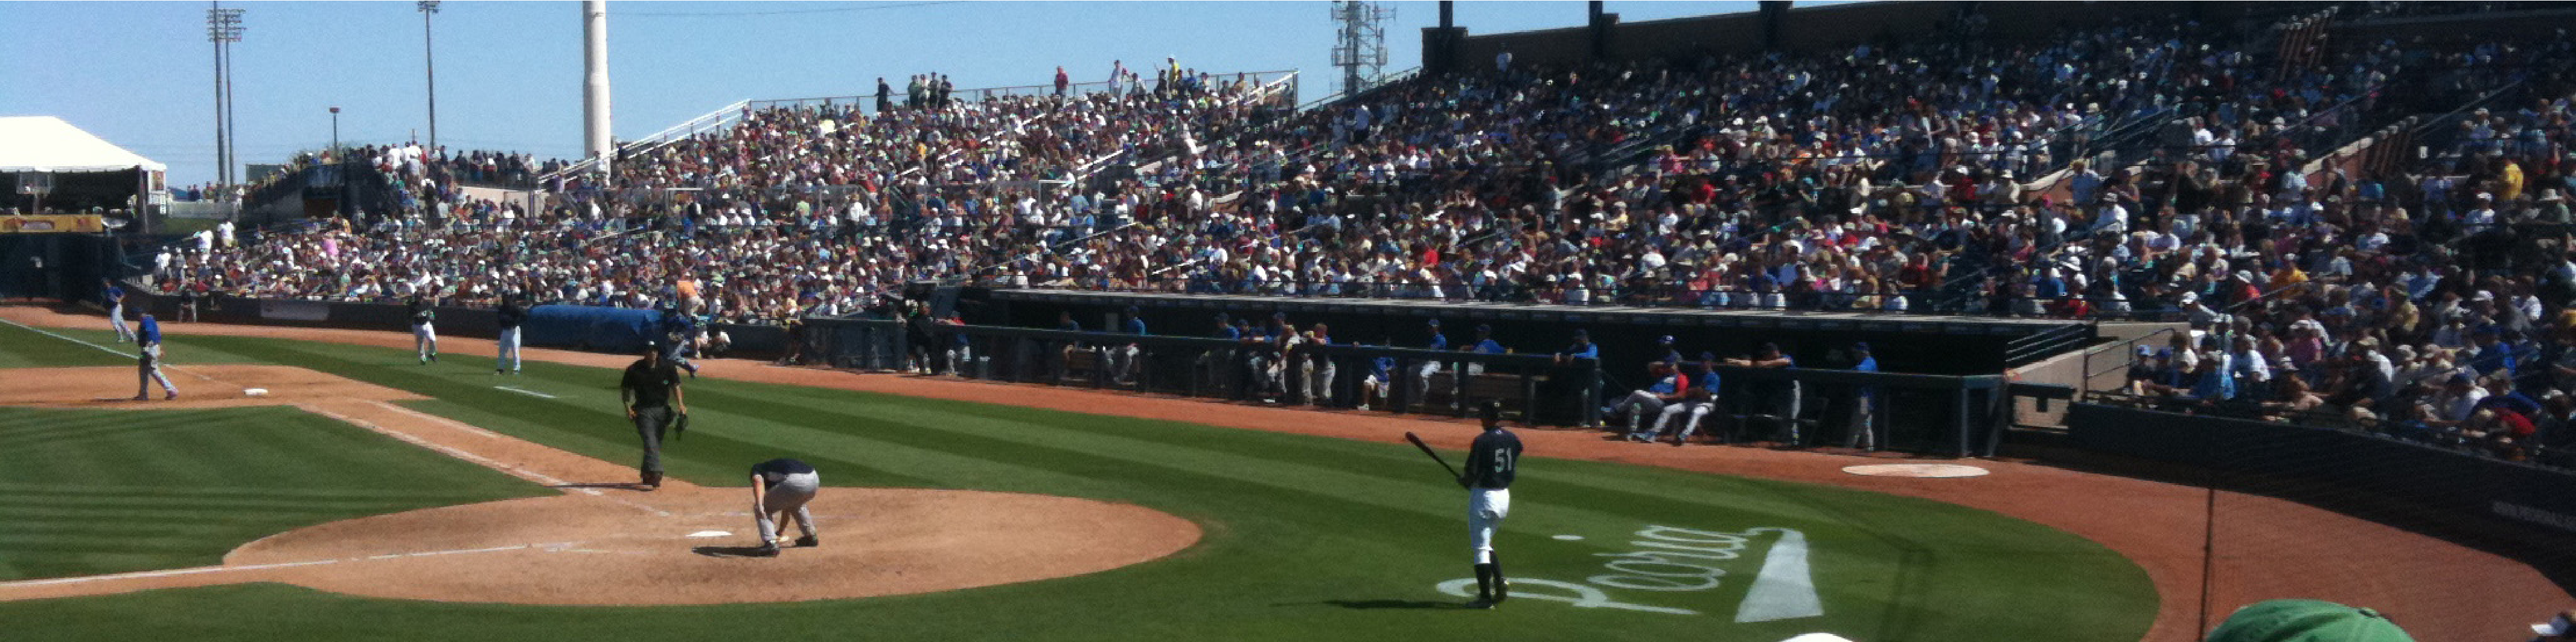
\includegraphics[width=\textwidth]{images/sampleteaser.pdf}
  \caption{Seattle Mariners at Spring Training, 2010.}
  \Description{Enjoying the baseball game from the third-base
  seats. Ichiro Suzuki preparing to bat.}
  \label{fig:teaser}
\end{teaserfigure}

%%
%% This command processes the author and affiliation and title
%% information and builds the first part of the formatted document.
\maketitle


% THIS IS THE MAIN PARTS OF THE DOCUMENT
\section{Introduction}
Code quality can be subjective, each person and organisation will have differing needs and wants when it comes to the quality of their code. But there are a many well defined areas that are as universal as can be.

test test
1234 aaa bbbb
\subsection{Secondary Part}
This is \textbf{another} part of my \textit{introduction}.

\begin{enumerate}
    \item This is the first item
    \item This is the second item
\end{enumerate}

This is another line of text that will go here

\begin{itemize}
  \item List entries start with the \verb|\item| command.
  \item Individual entries are indicated with a black dot, a so-called bullet.
  \item The text in the entries may be of any length.
\end{itemize}

\begin{table}[h]
\begin{tabular}{lll}
\hline
Colour & Score & Rating \\ \hline
Red    & 5     & B+     \\
Green  & 8     & A      \\ \hline
\end{tabular}
\end{table}
\section{Another Section}

Your section text goes here. Here is my citation \cite{ekkel2017nearby}. This is a cross reference to Figure \ref{fig:teaser}.

\begin{figure}[h]
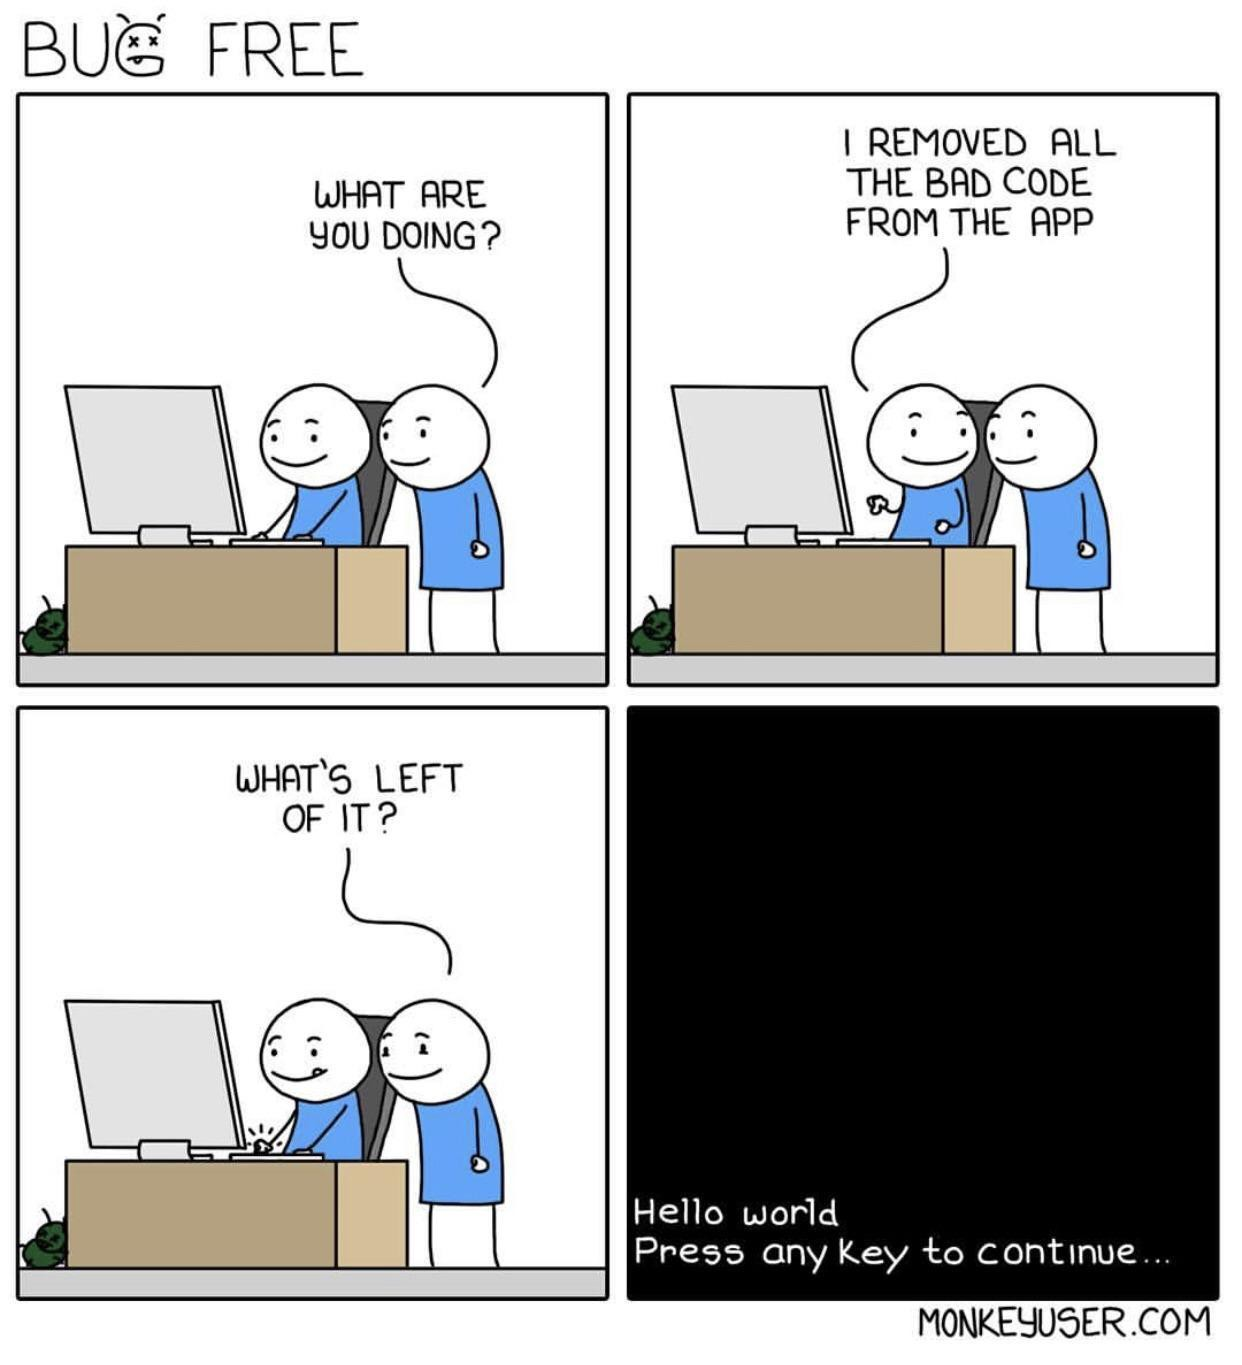
\includegraphics[width=\columnwidth]{images/code_all_gone.jpg}
\caption{A Picture of a Car}
\end{figure}

Lorem ipsum dolor sit amet, consectetur adipiscing elit. In orci nibh, vestibulum eget sodales quis, facilisis sed enim. Morbi at vehicula ipsum. Proin ornare ultrices enim, id cursus orci condimentum nec. Vestibulum condimentum maximus scelerisque. Nam ante neque, pellentesque ut facilisis vel, venenatis vitae orci. Lorem ipsum dolor sit amet, consectetur adipiscing elit. Maecenas ullamcorper sed turpis sit amet lacinia. Fusce imperdiet luctus erat. Sed ut est a purus tempus sodales interdum vitae purus. Ut sit amet sem viverra leo eleifend sollicitudin a at felis. Nunc eget rutrum nisi. Fusce consectetur blandit nibh. Nullam gravida scelerisque rutrum. Cras mattis aliquet turpis, et condimentum libero euismod sed. Integer enim mi, elementum eu pretium in, interdum a magna.

Nam vel consectetur odio. Curabitur cursus hendrerit mi, id bibendum augue vulputate sed. Vestibulum aliquam ullamcorper maximus. Aenean lacinia interdum commodo. Praesent eget laoreet est, maximus porta metus. Nulla commodo libero ut odio aliquet feugiat quis sit amet nisi. Duis eget aliquet neque.

Cras tempus dignissim elementum. Etiam nibh libero, condimentum id ornare at, rutrum in elit. Etiam eu metus eget neque vulputate ornare. Nam vel ex quis justo pharetra consequat ac vitae diam. Quisque et semper leo. Class aptent taciti sociosqu ad litora torquent per conubia nostra, per inceptos himenaeos. Suspendisse potenti. Nam magna nisl, pretium nec mauris convallis, blandit convallis metus. Nullam non diam vitae quam accumsan porttitor ac in mi. Nulla condimentum pretium venenatis. Suspendisse potenti. Morbi laoreet nibh quis nisl vulputate, eget elementum velit vehicula. Phasellus malesuada eleifend ligula et luctus. Mauris fringilla libero sit amet nibh imperdiet efficitur. Fusce quis tincidunt risus.

Nullam metus velit, porttitor sit amet orci eu, molestie scelerisque nibh. Duis urna massa, faucibus ut eros vitae, maximus ultricies nisi. Phasellus iaculis odio a eros aliquam, auctor fringilla risus euismod. Etiam metus diam, suscipit vel pellentesque quis, euismod a lacus. Nulla vitae aliquam tellus, vitae interdum sapien. Maecenas ultricies et odio et mattis. Aliquam erat volutpat. Aenean justo mi, congue eget tincidunt tincidunt, feugiat mollis ligula. Ut consectetur, lectus vel euismod dictum, sapien magna pellentesque est, vitae mollis odio tellus nec felis. Quisque eu tortor viverra, facilisis metus id, blandit dui. Proin sed laoreet ex. Nam suscipit non nisi sed eleifend. Cras dignissim diam eget nisl dictum aliquet vel ut tortor.

Etiam ac sapien risus. Aliquam ut enim dui. Pellentesque habitant morbi tristique senectus et netus et malesuada fames ac turpis egestas. Aliquam varius quam non leo hendrerit, vitae egestas leo scelerisque. Curabitur lacinia purus viverra justo venenatis tempor. Nunc at elit at erat pellentesque pulvinar at vel mauris. Aenean non urna eu urna dignissim placerat nec eu ipsum. Sed in nibh tincidunt, suscipit orci eu, finibus massa. Morbi euismod ante mauris, et faucibus magna lacinia eget. Nullam bibendum diam ligula, nec euismod sapien rhoncus vitae. Aenean aliquet condimentum sodales. Sed justo nunc, lacinia fermentum magna id, tempus vehicula dolor. In vitae pulvinar sem, nec congue ex.


\section{Yet Another Section}

Your section text goes here. I am goign to talk about accessibility \cite{jones1981accessibility}. And a second reference \cite{10.1145/1090785.1090831}.



%%
%% The acknowledgments section is defined using the "acks" environment
%% (and NOT an unnumbered section). This ensures the proper
%% identification of the section in the article metadata, and the
%% consistent spelling of the heading.
\begin{acks}
To Robert, for the bagels and explaining CMYK and color spaces.
\end{acks}

%%
%% The next two lines define the bibliography style to be used, and
%% the bibliography file.
\bibliographystyle{ACM-Reference-Format}
\bibliography{references}

%%
%% If your work has an appendix, this is the place to put it.
\appendix


\huge{\textbf{Appendices}}
\newline
\normalsize{Each appendix can be found either as a \underline{LINK} or in the sub folder with it's label, e.g. Appendix A is found in the path "/A/"}
\section{Control Flow Graph}
\section{Code Analyser Diagram}
\section{Compiler Diagram}
\section{User Personas}
\section{User Stories}
\section{Github Issues}
\url{https://github.com/aliveSurfin/code_quality/issues}
\section{MoSCoW Analysis}
\url{https://github.com/aliveSurfin/code_quality/projects/1}
\section{Value Risk}
\url{https://github.com/aliveSurfin/code_quality/projects/2}
\section{Combined MoscowValueRisk Priorities}
\url{https://github.com/aliveSurfin/code_quality/projects/3}
\section{T-Shirt Sizing}
\url{https://github.com/aliveSurfin/code_quality/projects/4}
\section{Source Code}
\url{https://github.com/aliveSurfin/code_quality/blob/main/development/code}
\section{Left Most Derivation Diagram}
\section{Right Most Derivation Diagram}
\section{Code Editor Initial Designs}
\section{Parser}
\url{https://github.com/aliveSurfin/code_quality/blob/main/development/code/parsing/parser/Parser.js}
\section{AST Types}
\url{https://github.com/aliveSurfin/code_quality/blob/main/development/code/parsing/parser/AST_CONST_TYPES.js}
\section{Tokeniser Folder}
\url{https://github.com/aliveSurfin/code_quality/tree/main/development/code/parsing/tokenizer}
\section{Parser Tests}
\url{https://github.com/aliveSurfin/code_quality/tree/main/development/code/parsing/parser/tests}
\section{Development Diary}
\url{https://github.com/aliveSurfin/code_quality/blob/main/development/diary/diary.md}
\section{Evaluation Features}
\url{https://github.com/aliveSurfin/code_quality/tree/main/development/code/parsing/evaluate}
\section{Final Product}
\url{https://code-quality-honours.herokuapp.com/}
\section{Code Coverage}
\section{Interview Notes}
\section{User Testing Results}


\end{document}
\endinput
%%
%% End of file `sample-sigconf.tex'.
